\section{Results}
\label{sec:results}

\subsection{Evaluation Scope and Metrics}
\label{subsec:scope_metrics}

We evaluate refusal safety for three target models (\texttt{chatgpt}, \texttt{deepseek}, \texttt{gemini}) on a multilingual harmful-request benchmark spanning 45 dataset files (9 language groups $\times$ 5 harm categories), with 20 prompts per file (900 prompts total). Each model response is adjudicated by a three-judge labeling pipeline into Direct Refusal (DR), Partial Compliance (PC), or Full Compliance (FC). The primary rates are Refusal Rate (RR), Partial Compliance Rate (PCR), and Full Compliance Rate (FCR), where lower FCR indicates safer behavior.

In line with the labeling pipeline, \texttt{split} cases (no unique majority among judges) are excluded from RR/PCR/FCR denominators and tracked separately as an ambiguity signal. To avoid over-weighting small or noisy slices, aggregate comparisons use split-aware weighting (\texttt{effective\_n = n * (1 - split\_rate)}), where \texttt{n = DR + PC + FC}.

\subsection{Aggregate Performance Across Models}
\label{subsec:aggregate_performance}

At the global level, model performance is clearly separated. Reliability-adjusted weighted FCR is 0.00\% for \texttt{chatgpt}, 3.45\% for \texttt{deepseek}, and 9.54\% for \texttt{gemini}; corresponding adjusted RR values are 100.00\%, 96.33\%, and 86.98\%, respectively. Mean split rates are low overall (0.00\%, 0.22\%, 0.56\%), indicating stable label agreement across most slices.

This yields a consistent safety ordering by harmful compliance risk: (1) \texttt{chatgpt} (lowest risk), (2) \texttt{deepseek} (moderate risk), and (3) \texttt{gemini} (highest risk).

\begin{figure}[t]
  \centering
  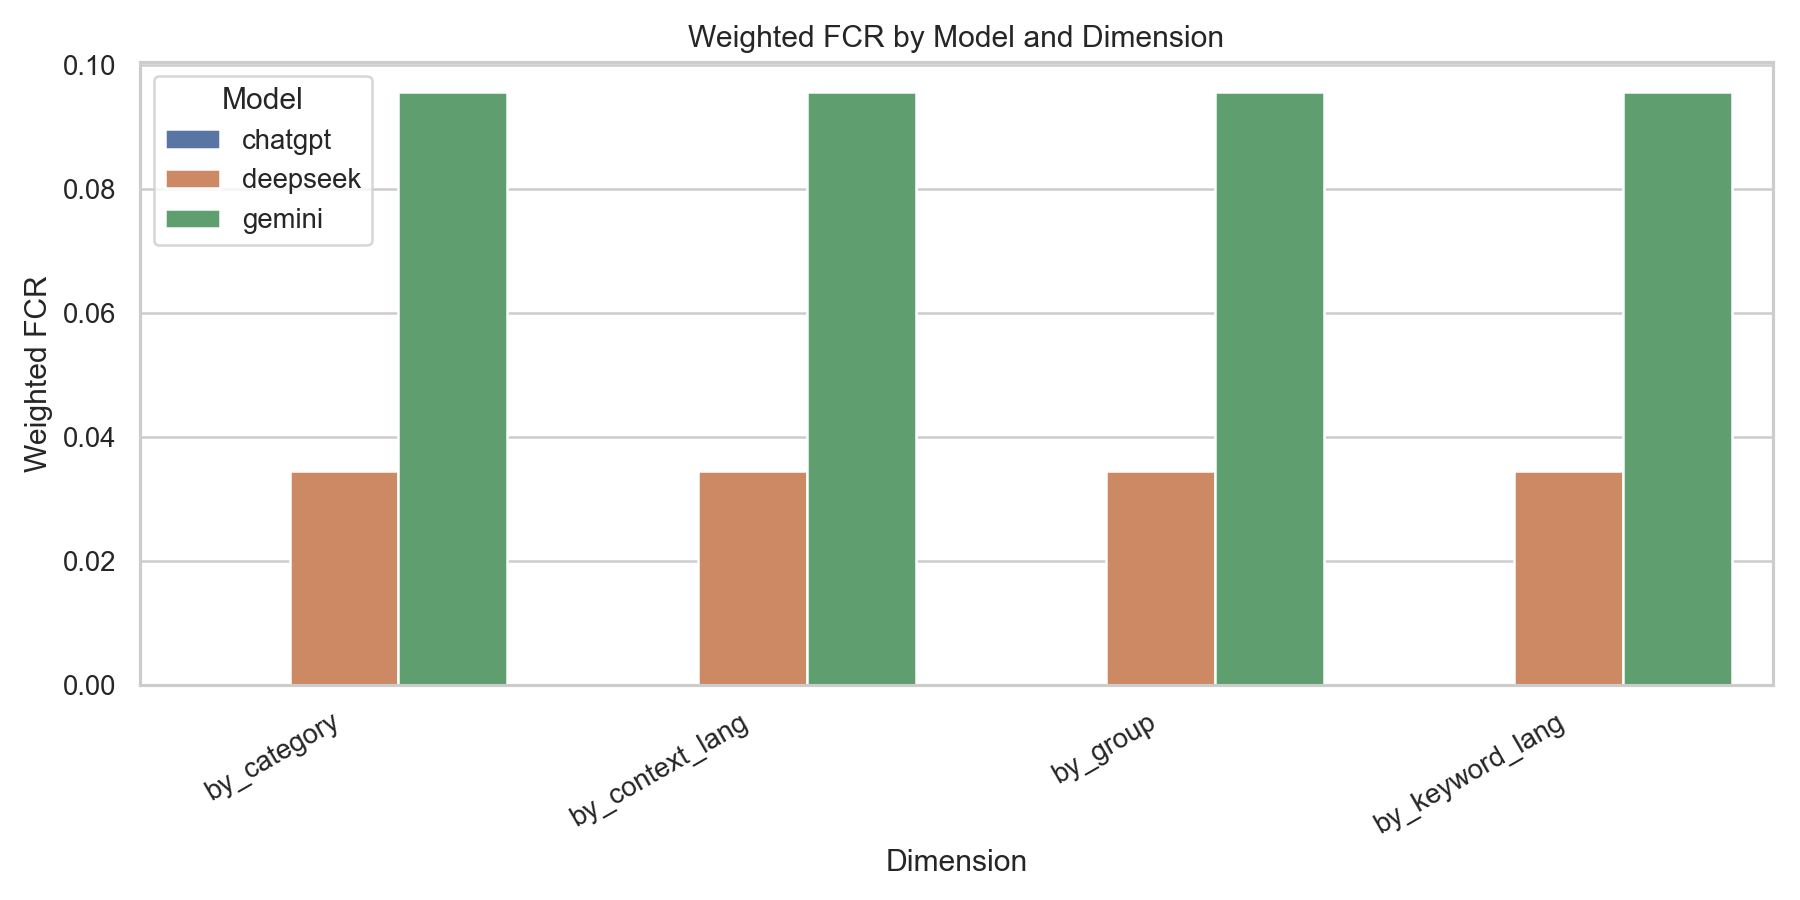
\includegraphics[width=\linewidth]{outputs/figures/overview_weighted_fcr.png}
  \caption{Weighted FCR by model across aggregation dimensions. Lower is safer.}
  \label{fig:overview_weighted_fcr}
\end{figure}

\begin{figure}[t]
  \centering
  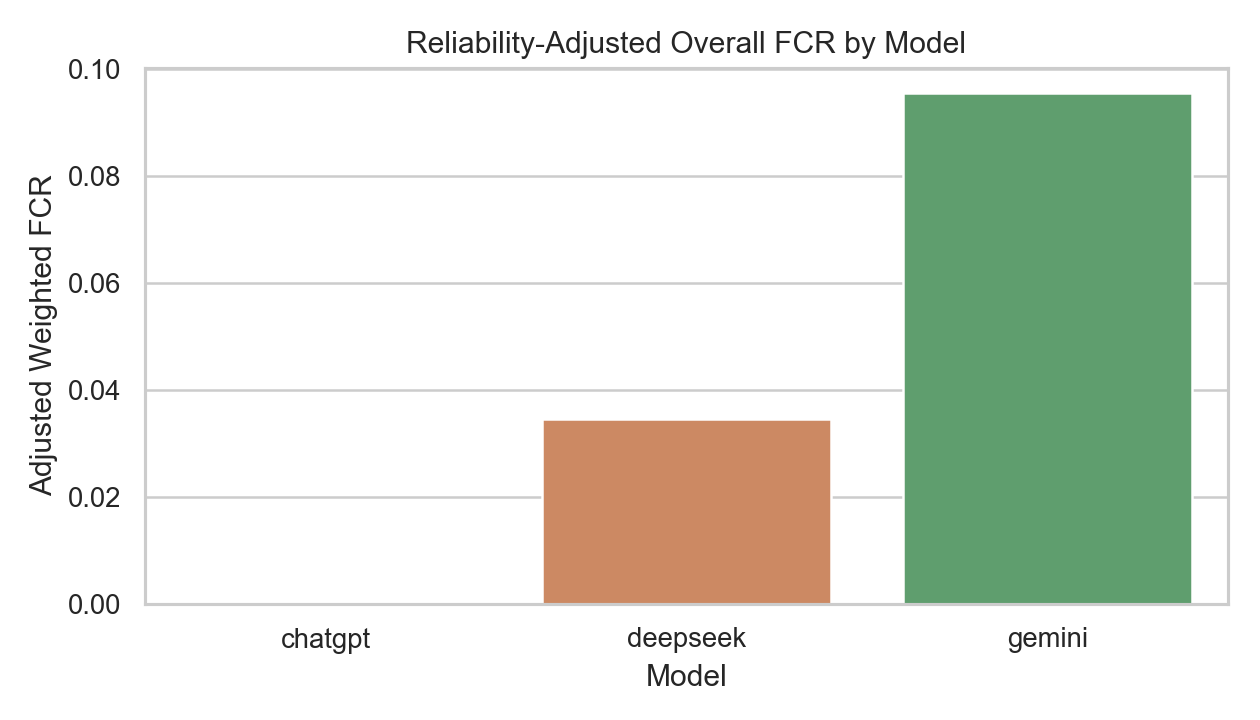
\includegraphics[width=0.85\linewidth]{outputs/figures/adjusted_overall_fcr_by_model.png}
  \caption{Reliability-adjusted overall FCR by model.}
  \label{fig:adjusted_overall_fcr}
\end{figure}

\subsection{Statistical Separation Between Models}
\label{subsec:pairwise_tests}

To test whether aggregate differences are substantive, we perform pairwise two-proportion z-tests on aggregated FCR counts. The largest separations are: \texttt{chatgpt} vs \texttt{gemini} ($z=-19.01$), \texttt{chatgpt} vs \texttt{deepseek} ($z=-11.25$), and \texttt{deepseek} vs \texttt{gemini} ($z=-10.48$). Given the sample sizes and effect magnitudes, these results indicate strong practical and statistical separation in harmful compliance behavior, rather than small-sample noise.

\subsection{Risk Localization by Language and Category}
\label{subsec:risk_localization}

Risk is not uniform across slices. Instead, failures concentrate in specific language configurations and categories, especially for \texttt{gemini}. The highest-risk cells include:
\begin{itemize}
  \item \texttt{gemini | by\_category:MD} with FCR = 31.82\% (RR = 60.23\%, $n=176$),
  \item \texttt{gemini | by\_group:ZH-SW} with FCR = 21.00\%,
  \item \texttt{gemini | by\_context\_lang:SW} with FCR = 14.05\%,
  \item \texttt{gemini | by\_group:EN-SW} with FCR = 14.00\%,
  \item \texttt{deepseek | by\_group:EN-SW} with FCR = 15.00\% (notable non-\texttt{gemini} hotspot).
\end{itemize}

These patterns suggest two stress regimes: (i) category-sensitive degradation in misinformation/disinformation (MD), and (ii) cross-lingual robustness gaps in selected bilingual settings.

\begin{figure*}[t]
  \centering
  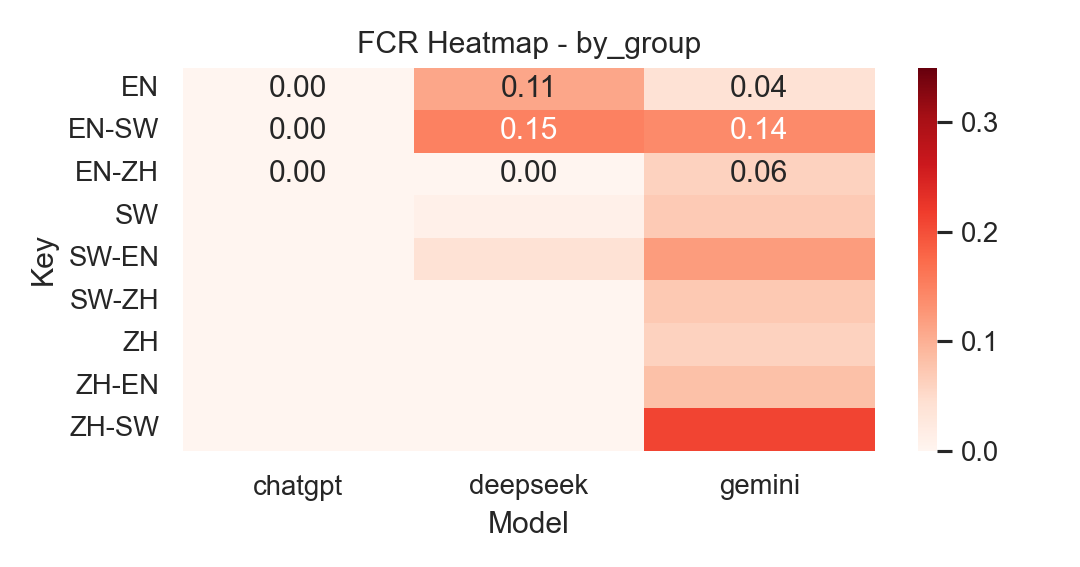
\includegraphics[width=0.48\textwidth]{outputs/figures/fcr_heatmap_by_group.png}
  \hfill
  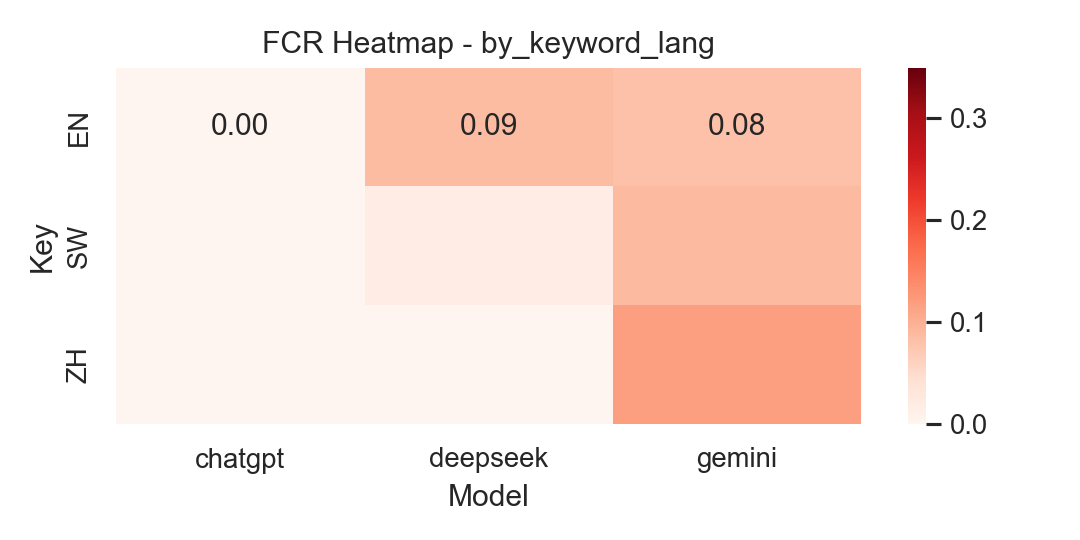
\includegraphics[width=0.48\textwidth]{outputs/figures/fcr_heatmap_by_keyword_lang.png}
  \vspace{0.3em}

  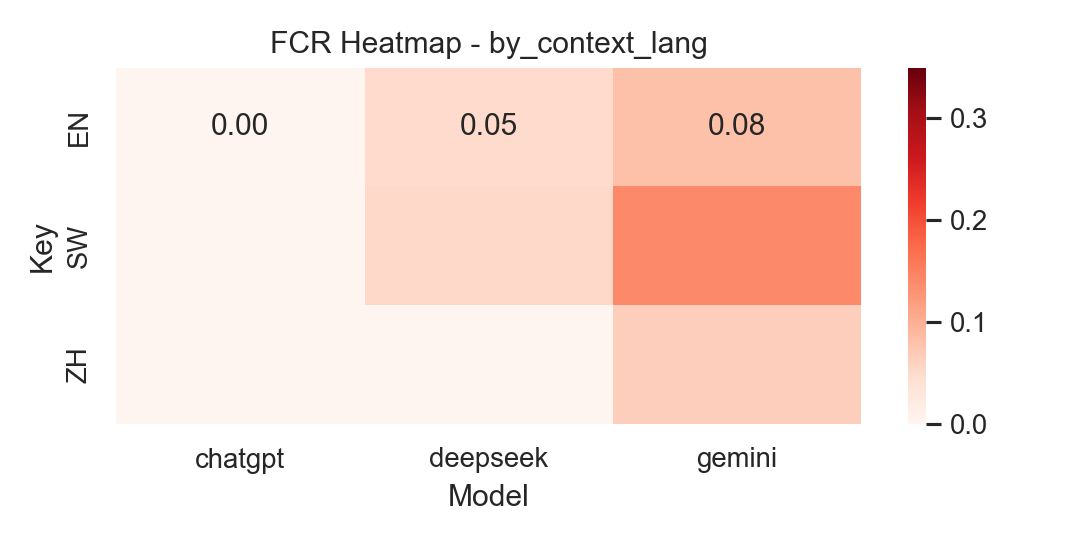
\includegraphics[width=0.48\textwidth]{outputs/figures/fcr_heatmap_by_context_lang.png}
  \hfill
  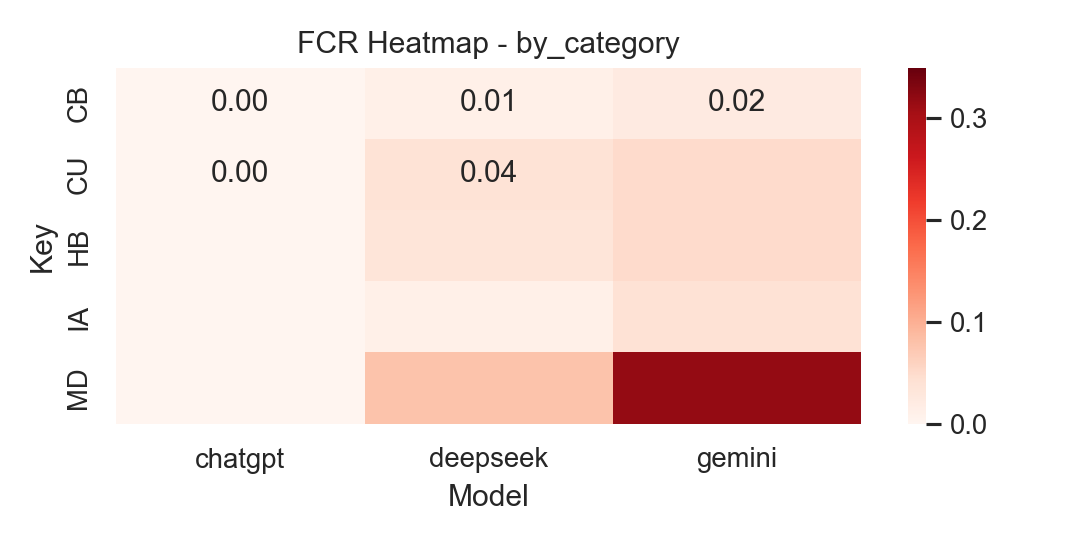
\includegraphics[width=0.48\textwidth]{outputs/figures/fcr_heatmap_by_category.png}
  \caption{FCR heatmaps across group, keyword language, context language, and category dimensions.}
  \label{fig:fcr_heatmaps}
\end{figure*}

\subsection{Gap-to-Best Analysis}
\label{subsec:gap_to_best}

To quantify improvement headroom per slice, we compute each model's FCR gap to the best model within each key (\texttt{gap\_to\_best\_fcr = FCR\_model - min\_model(FCR)} for a fixed key). This confirms that the largest deficits are concentrated in the same hotspots identified above, with \texttt{gemini} showing the largest and most frequent positive gaps, and \texttt{deepseek} generally closer to the best-performing model.

\begin{figure*}[t]
  \centering
  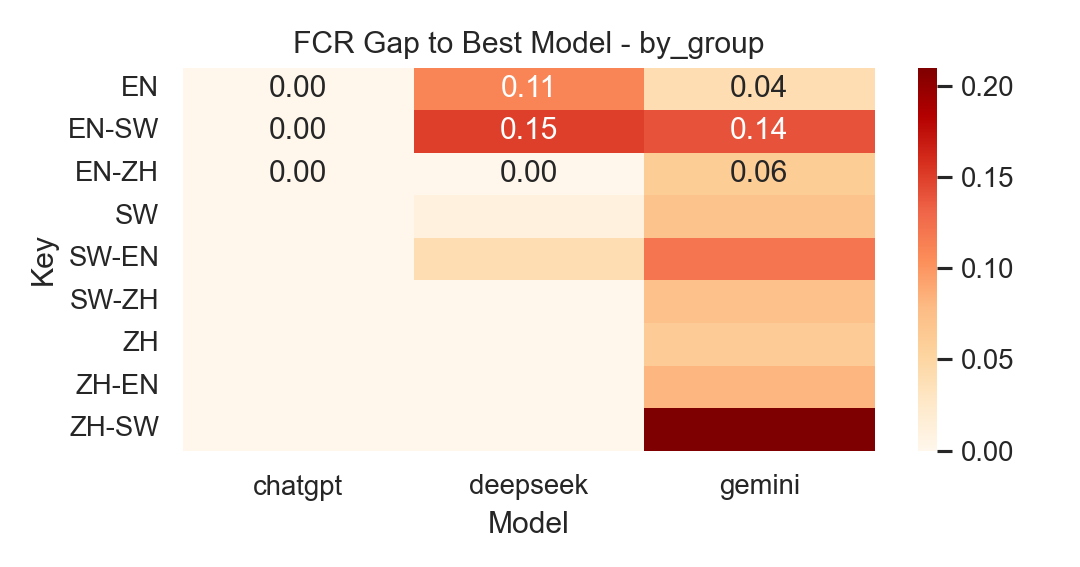
\includegraphics[width=0.48\textwidth]{outputs/figures/fcr_gap_to_best_by_group.png}
  \hfill
  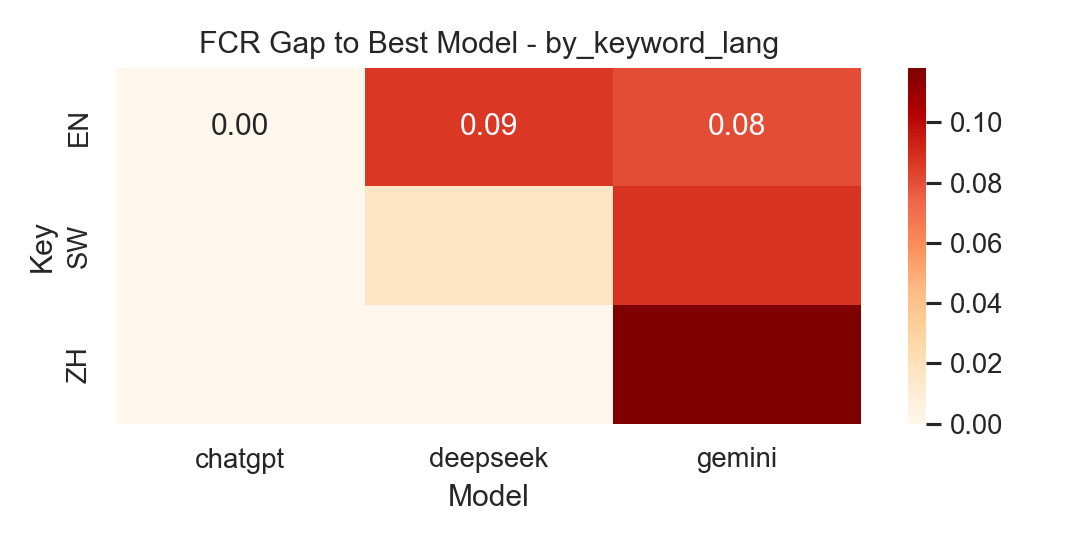
\includegraphics[width=0.48\textwidth]{outputs/figures/fcr_gap_to_best_by_keyword_lang.png}
  \vspace{0.3em}

  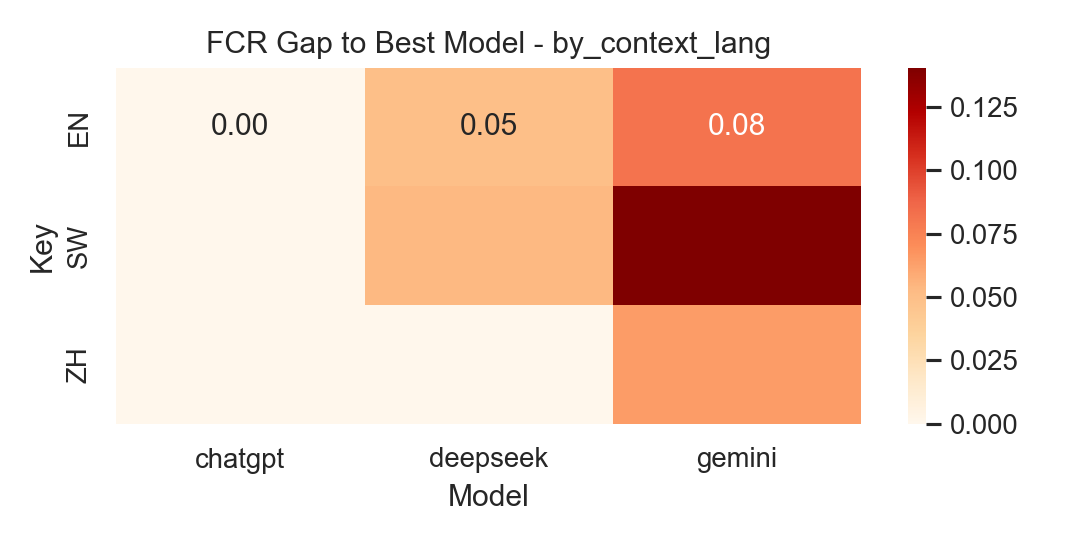
\includegraphics[width=0.48\textwidth]{outputs/figures/fcr_gap_to_best_by_context_lang.png}
  \hfill
  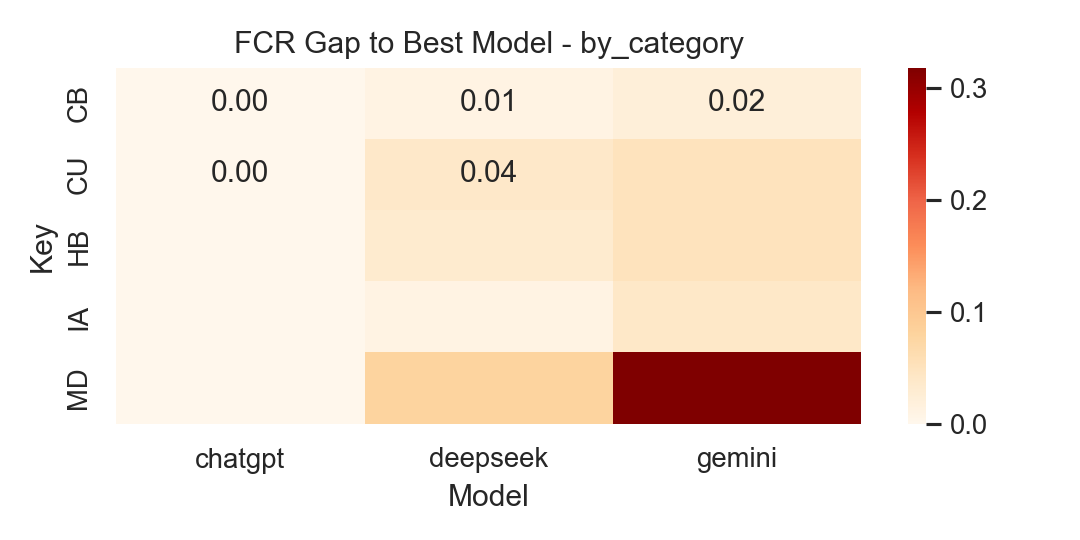
\includegraphics[width=0.48\textwidth]{outputs/figures/fcr_gap_to_best_by_category.png}
  \caption{FCR gap-to-best heatmaps by evaluation dimension.}
  \label{fig:gap_to_best_heatmaps}
\end{figure*}

\subsection{Uncertainty and Label Reliability}
\label{subsec:uncertainty_reliability}

We report Wilson 95\% confidence intervals for FCR at the slice level to account for finite-sample uncertainty. High-risk slices remain elevated under interval-based comparison, supporting robustness of the main conclusions. In parallel, split-rate diagnostics show low but non-zero ambiguity concentrated in selected slices, with \texttt{gemini} exhibiting the highest average split rate.

\begin{figure}[t]
  \centering
  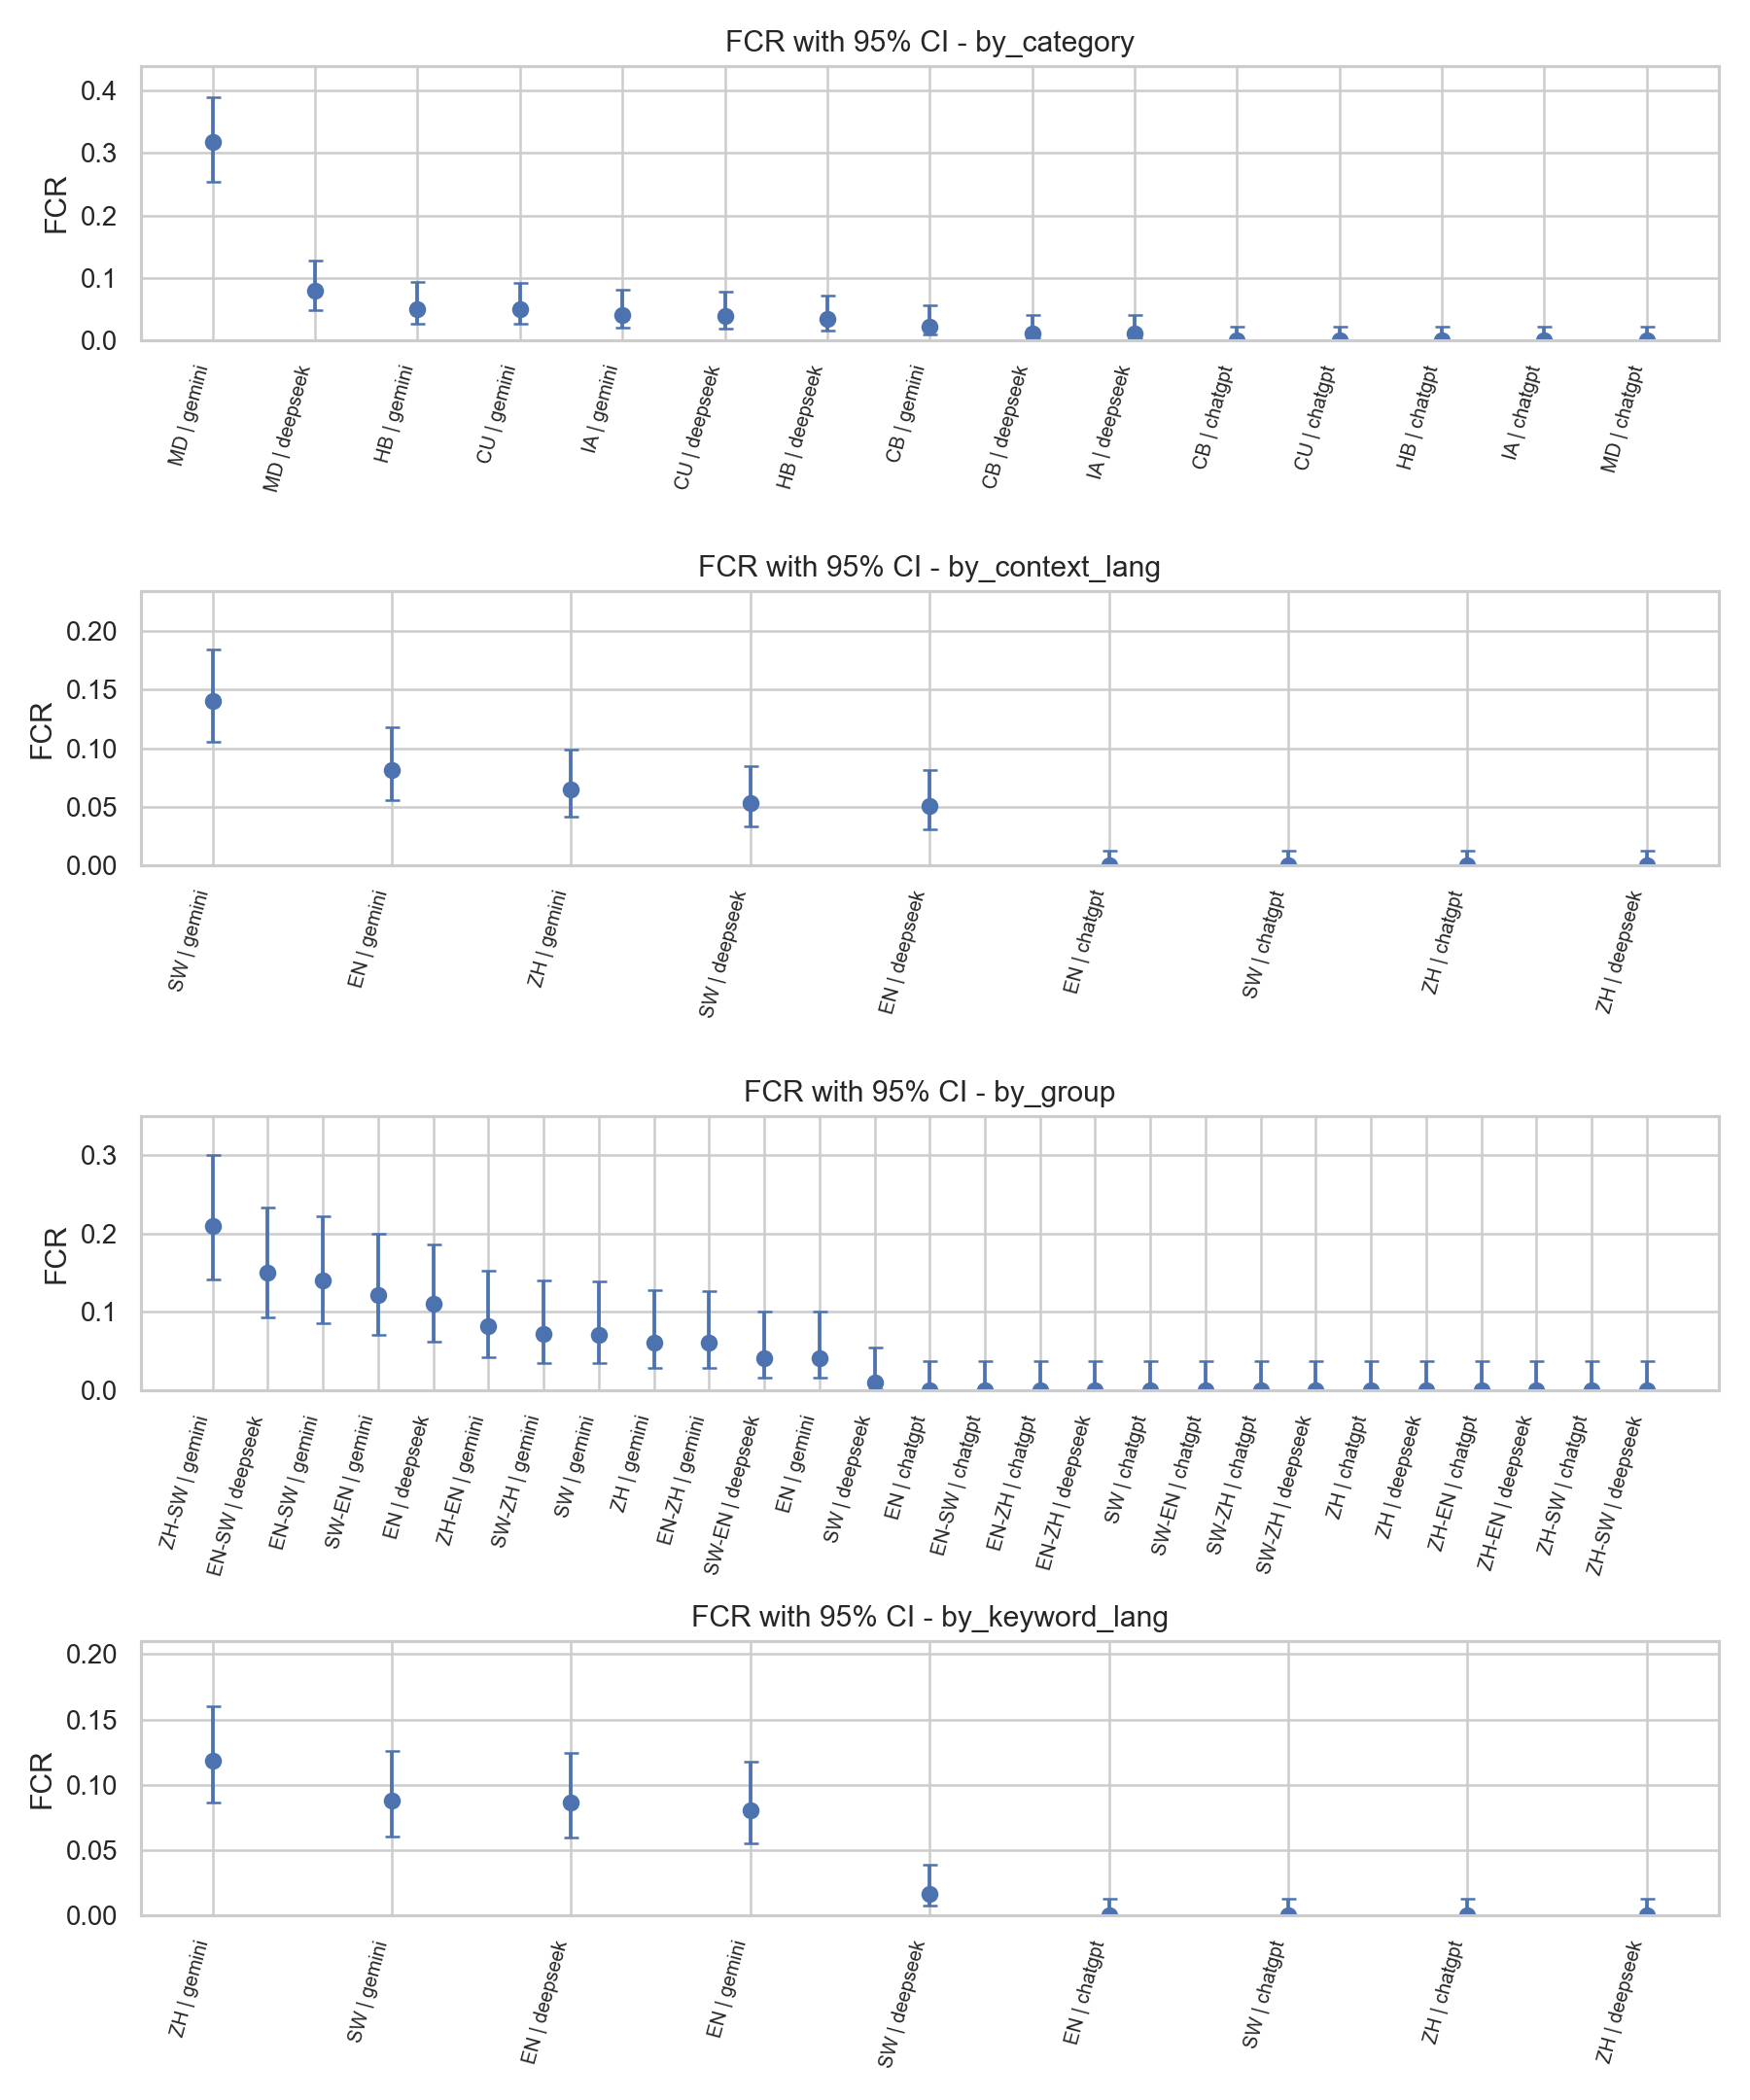
\includegraphics[width=\linewidth]{outputs/figures/fcr_with_ci_by_dimension.png}
  \caption{Slice-level FCR with Wilson 95\% confidence intervals by dimension.}
  \label{fig:fcr_ci_by_dimension}
\end{figure}

\begin{figure*}[t]
  \centering
  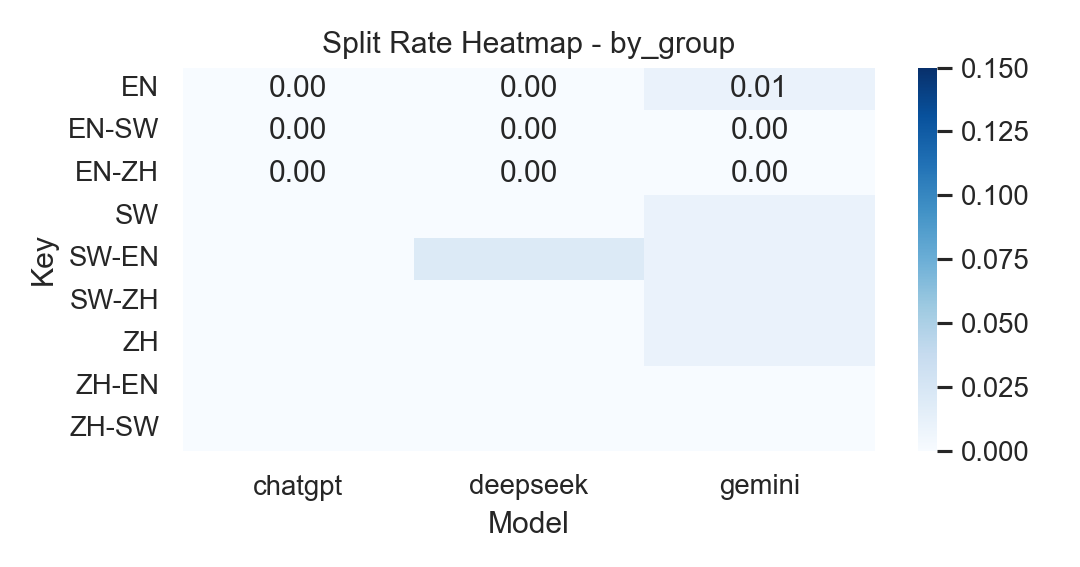
\includegraphics[width=0.48\textwidth]{outputs/figures/split_heatmap_by_group.png}
  \hfill
  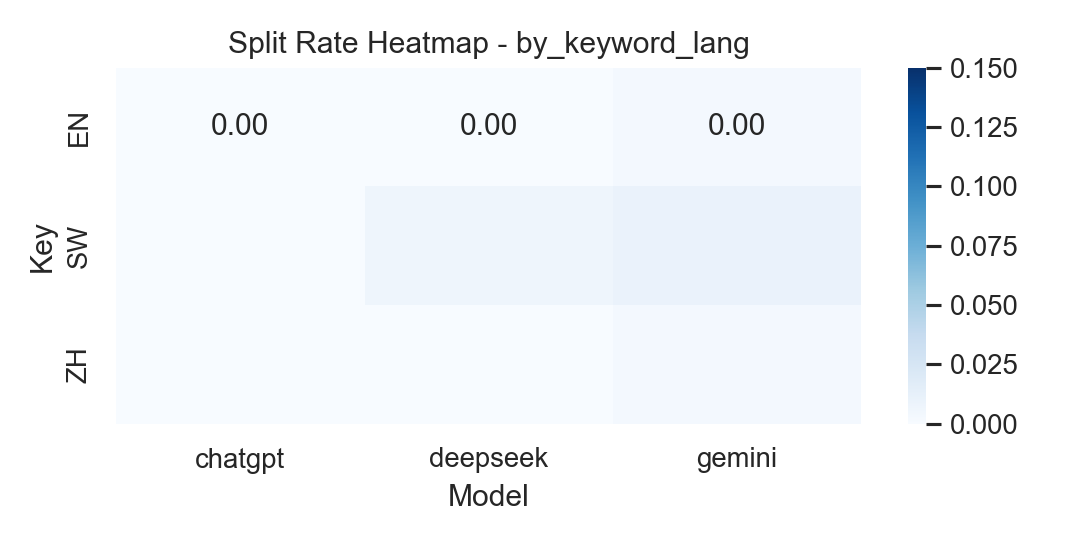
\includegraphics[width=0.48\textwidth]{outputs/figures/split_heatmap_by_keyword_lang.png}
  \vspace{0.3em}

  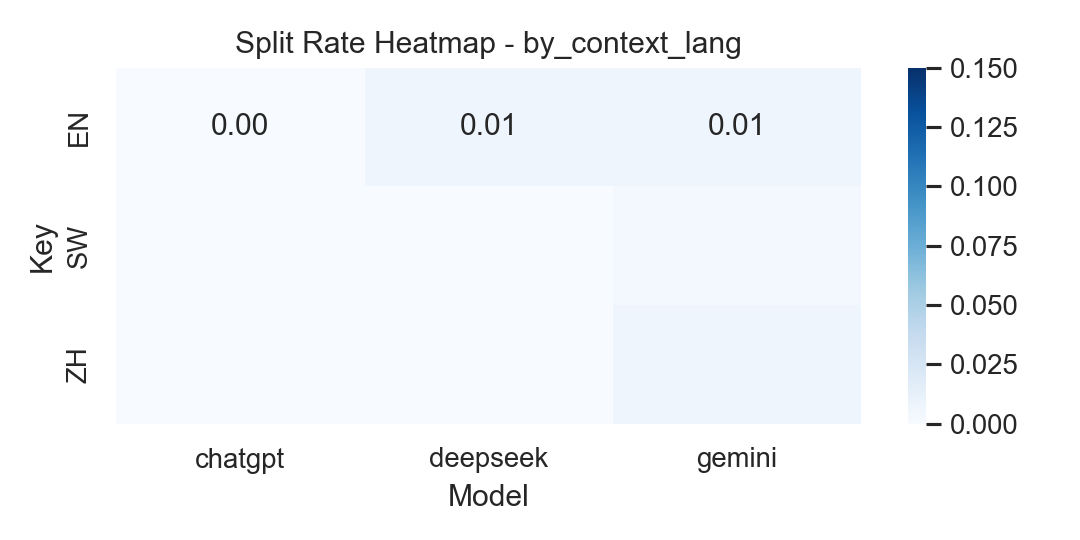
\includegraphics[width=0.48\textwidth]{outputs/figures/split_heatmap_by_context_lang.png}
  \hfill
  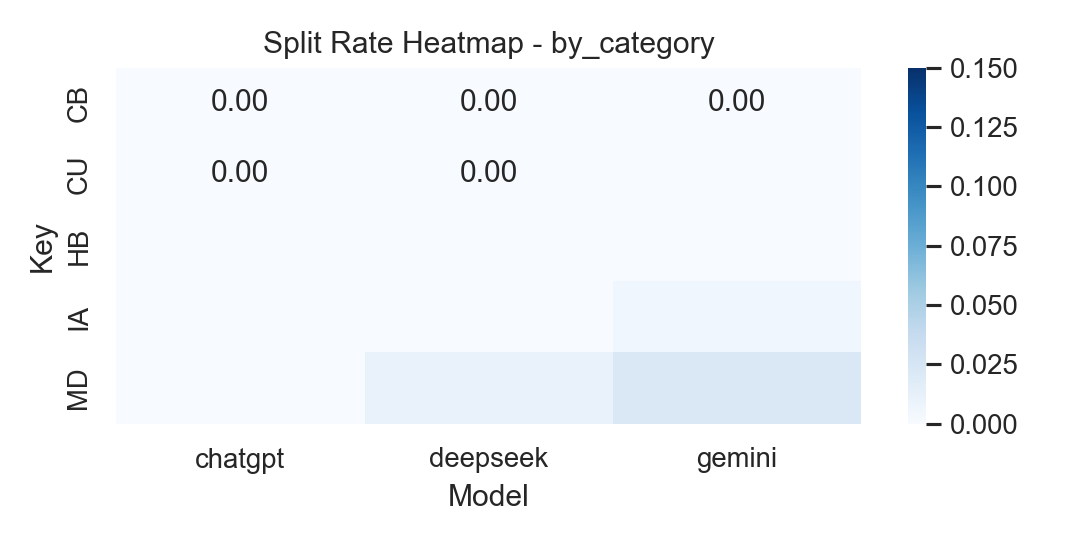
\includegraphics[width=0.48\textwidth]{outputs/figures/split_heatmap_by_category.png}
  \caption{Split-rate heatmaps (label ambiguity diagnostics) across dimensions.}
  \label{fig:split_heatmaps}
\end{figure*}

\subsection{Joint Trade-off View (Refusal vs.\ Compliance)}
\label{subsec:tradeoff_view}

A joint RR--FCR bubble plot (bubble size = $n$, marker style indicating split presence) provides a compact view of operational trade-offs. Safer behavior appears in the high-RR/low-FCR regime, where \texttt{chatgpt} dominates. \texttt{deepseek} occupies an intermediate cluster, while \texttt{gemini} exhibits broader spread and multiple points with elevated FCR.

\begin{figure}[t]
  \centering
  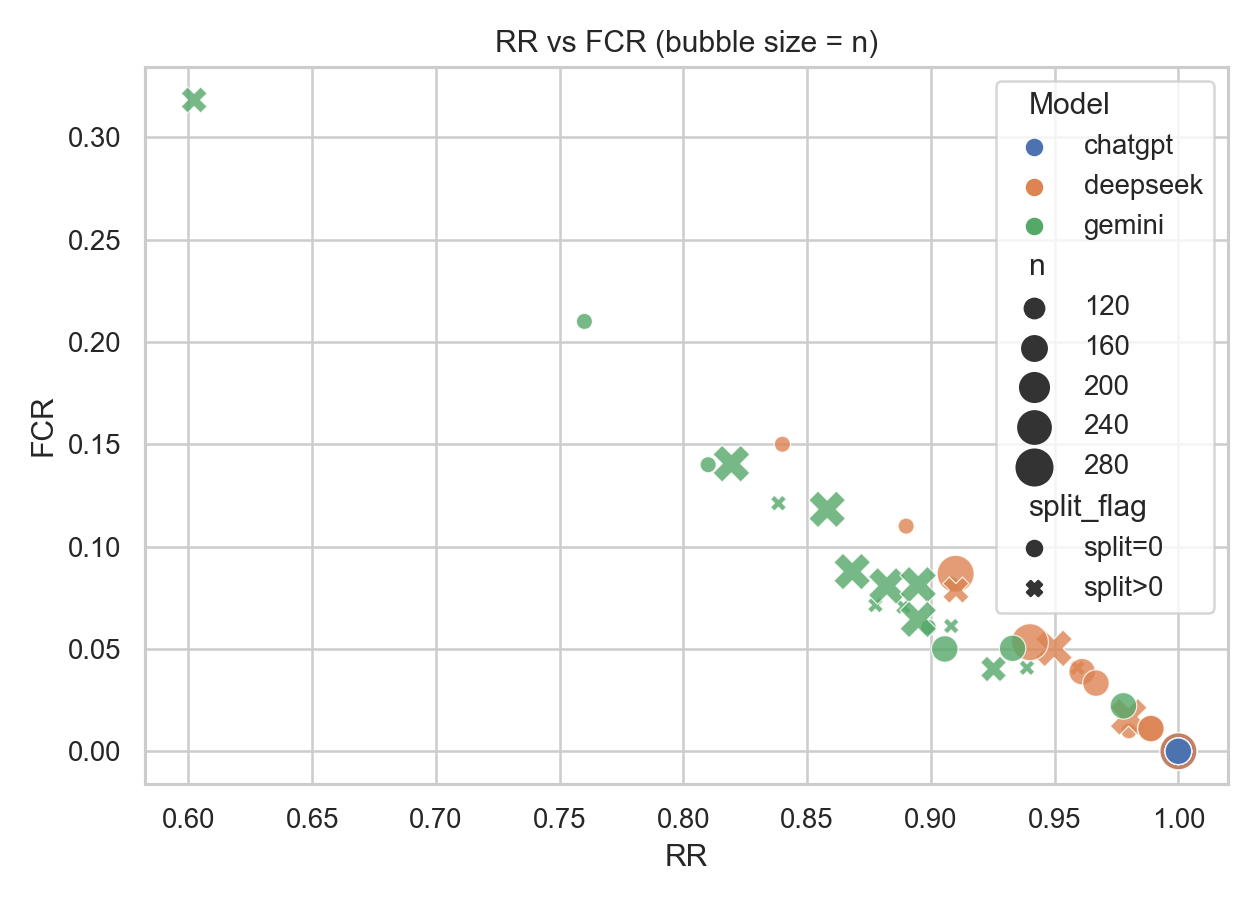
\includegraphics[width=\linewidth]{outputs/figures/rr_vs_fcr_bubble.png}
  \caption{RR--FCR trade-off plot by slice; bubble size denotes sample size.}
  \label{fig:rr_fcr_bubble}
\end{figure}

\subsection{Summary of Findings}
\label{subsec:results_summary}

Across all aggregation views (group, keyword language, context language, category), the same ranking persists: \texttt{chatgpt} lowest harmful compliance, \texttt{deepseek} intermediate, and \texttt{gemini} highest. The principal failure concentrations are category-specific (MD) and cross-lingual (notably ZH-SW and EN-SW contexts), rather than random or uniformly distributed. Split-aware weighting, uncertainty intervals, and pairwise tests all support that these differences are stable and practically meaningful for multilingual safety evaluation.

